\title{FYS-STK4155 \\
Project 1}
\author{Lars Johan Brodtkorb}
\date{ }

\subsection*{Abstract}

In this exercise I have tried to figure out which method is to be preferred of ordinary least squares, Ridge and Lasso regressions. The results show a better prediction error for the ridge regression, but that may be due to a faulty implementation of the Lasso method. 

\section{Introduction}

The main aim of this project is to study in more detail various
regression methods, including the Ordinary Least Squares (OLS) method,
Ridge regression and finally Lasso regression.
The methods are in turn combined with resampling techniques.

We will first study how
to fit polynomials to a specific two-dimensional function called
\href{{http://www.dtic.mil/dtic/tr/fulltext/u2/a081688.pdf}}{Franke's
	function}.  This
is a function which has been widely used when testing various  interpolation and fitting
algorithms. Furthermore, after having etsablished the model and the
method, we will employ resampling techniques such as the  cross-validation and/or
the bootstrap methods, in order to perform a proper assessment of our models.


The Franke function, which is a weighted sum of four exponentials  reads as follows
\begin{align*}
f(x,y) &= \frac{3}{4}\exp{\left(-\frac{(9x-2)^2}{4} - \frac{(9y-2)^2}{4}\right)}+\frac{3}{4}\exp{\left(-\frac{(9x+1)^2}{49}- \frac{(9y+1)}{10}\right)} \\
&+\frac{1}{2}\exp{\left(-\frac{(9x-7)^2}{4} - \frac{(9y-3)^2}{4}\right)} -\frac{1}{5}\exp{\left(-(9x-4)^2 - (9y-7)^2\right) }.
\end{align*}

The function will be defined for $x,y\in [0,1]$.  Our first step will
be to perform an OLS regression analysis of this function, trying out
a polynomial fit with an $x$ and $y$ dependence of the form $[x, y,
x^2, y^2, xy, \dots]$. We will also include cross-validation and
bootstrap as resampling techniques.  As in homeworks 1 and 2, we
can use a uniform distribution to set up the arrays of values for $x$
and $y$, or as in the example below just a fix values for $x$ and $y$ with a given step size.
In this case we will have two predictors and need to fit a
function (for example a polynomial) of $x$ and $y$.  Thereafter we will
repeat much of the same procedure using the the Ridge and
Lasso regression methods, introducing thus a dependence on the bias
(penalty) $\lambda$.

Thereafter we are going to use (real) digital terrain data and try to
reproduce these data using the same methods. We will also try to go
beyond the second-order polynomials metioned above and explore 
which polynomial fits the data best.


\section{Methods}


\subsection{Measures of prediction accuracy}

Find the confidence intervals of the $\beta$ parameters by computing their variances, evaluate the Mean Squared error (MSE)
\[ MSE(\hat{y},\hat{\tilde{y}}) = \frac{1}{n}
\sum_{i=0}^{n-1}(y_i-\tilde{y}_i)^2, 
\] 
and the $R^2$ score function.
If $\tilde{\hat{y}}_i$ is the predicted value of the $i-th$ sample and $y_i$ is the corresponding true value, then the score $R^2$ is defined as
\[
R^2(\hat{y}, \tilde{\hat{y}}) = 1 - \frac{\sum_{i=0}^{n - 1} (y_i - \tilde{y}_i)^2}{\sum_{i=0}^{n - 1} (y_i - \bar{y})^2},
\]
where we have defined the mean value  of $\hat{y}$ as
\[
\bar{y} =  \frac{1}{n} \sum_{i=0}^{n - 1} y_i.
\]

\subsection{Ordinary least square regression}

We have an input vector $X^T = (X_1,X_2,X_3,...,X_p)$ and want to predict a real-valued output Y. The linear regression model has the form: (\cite{elementsstat}, chapter 3.2)

\begin{equation}
f(X) = \beta_0 + \sum_{j=1}^{p}X_j\beta_j
\end{equation}


The linear model either assumes that the regression function $E(Y |X)$ is
linear, or that the linear model is a reasonable approximation. The $\beta_j$ ’s are unknown parameters or coefficients, and the variables $X_j$ can come
from many different sources. One of them is that of basis expansions such as 

$X_2 = X_1^2, X_3 = X_1^3$, leading to a polynomial
representation;

We can use the basis expansions as a device to achieve more flexible representations for f(X). Polynomials are an example of this. Having great flexibility in approximation allows the basis expansions to work for many occurences, but their variability may increase heavily if they are applied outside their intended scope. The coefficients to achieve a functional form
in one region can cause the function to flap about madly in remote regions (\cite{elementsstat}, chapter 5.1, p. 140). 

The polynomial method produces a dictionary $D$ consisting of typically a very large number of basis functions $|D|$, far more than we can afford to fit to our data. Along
with the dictionary we require a method for controlling the complexity
of our model, using basis functions from the dictionary. There are three
common approaches:
Restriction, selection and regularization methods, which we will revisit in the Ridge and Lasso segment.


No matter the source of the $X_j$, the model is linear in the parameters. Typically we have a set of training data $(x_1, y_1)...(x_N , y_N )$ from which
to estimate the parameters $\beta$. Each $x_i = (x_{i1}, x_{i2},...,x_{ip})^T$ is a vector of feature measurements for the i-th case.

Using linear least squared fittings for $X \in \R^2$ we can get the linear function of X that minimizes the sum of the sum of squared residuals of Y.

A unique solution for $\beta$ has the form:

\begin{align*}
\beta =(\textbf{X}^T\textbf{X})^{-1}\textbf{X}^T\textbf{y}
\end{align*}
\medskip

We have made minimal assumptions about the true distribution
of the data. In order to pin down the sampling properties of $\hat{\beta}$ , we now
assume that the observations $y_i$ are uncorrelated and have constant variance
$\sigma^2$, and that the $x_i$ are fixed (non random). The $\hyphenation{variance covariance}$
matrix of the least squares parameter estimates is then given by:

\begin{align*}
Var(\hat{\beta}) =(\textbf{X}^T\textbf{X})^{-1}\sigma^2
\end{align*}
\medskip


\subsection{K-fold cross-validation algorithm}

Cross-validation is probably the simplest and most widely used method for estimating prediction
error. This method directly estimates the expected
extra-sample error $Err = E[L(Y, \hat{f(X)})]$, the average generalization error when the method $\hat{f(X)}$ is applied to an independent test sample from the joint distribution of X and Y. As mentioned earlier, we might hope that cross-validation estimates the conditional error, with the training set T held fixed. Unfortunately, cross-validation typically estimates well only the expected prediction error (\cite{elementsstat}, chapter 7.10 - 7.12).


K-fold crossvalidation uses part of the available data to fit the model, and a different part to test it. We split the data into K roughly equal-sized parts. For the kth part, we fit the model to the other $K-1$ parts of the data, and calculate the prediction error of the fitted model when predicting the kth part of the data. We do this for k = 1, 2,...,K and
combine the K estimates of prediction error.


Given a set of models $f(x,\alpha)$ indexed by a tuning parameter $\alpha$, denote 
$\hat{f}^{-\kappa(x,\alpha)}$ by the $\alpha$-th model fitted with the k-th part of the data removed. Then for this set of models we define:

\begin{equation}
CV(\hat{f},\alpha) = \frac{1}{N}\sum_{i=1}^{N}L(y_i,\hat{f}^{-\kappa(i)}(x_i,\alpha))
\end{equation}
\medskip

where L is the loss function, $\kappa$ is the removed data.

The function $CV(\hat{f},\alpha)$ provides an estimate of the test error curve, and we
find the tuning parameter $\hat{\alpha}$ that minimizes it. Our final chosen model is
$f(x,\hat{\alpha})$, which we then fit to all the data.
\medskip
\medskip

The steps of the cross-validation method: \newline
(a) Find a subset of “good” predictors that show fairly strong (univariate) correlation with the class labels, using all of the samples except those in fold k.\newline
(b) Using just this subset of predictors, build a multivariate classifier, using all of the samples except those in fold k.\newline
(c) Use the classifier to predict the class labels for the samples in
fold k.

\subsection{Bootstrap}

The bootstrap method has been used in this project to estimate the variance and bias.
As with cross-validation, the bootstrap seeks to estimate the conditional error, but typically estimates well only the expected prediction error.

Suppose we have a model fit to a set of training data. We denote the
training set by $Z = (z_1, z_2,...,z_N )$ where $z_i = (x_i, y_i).$ The basic idea is
to randomly draw datasets with replacement from the training data, each
sample the same size as the original training set. This is done B times
(B = 200 in my application), producing B bootstrap datasets.
Then we refit the model to each of the bootstrap datasets, and examine
the behavior of the fits over the B replications (\cite{elementsstat} p.249)




\subsection{Ridge and Lasso regression}

\subsubsection*{Ridge regression}
Ridge regression is a simple example of a regularization approach, while the lasso is both a regularization and selection method. 

Selection methods adaptively scan the dictionary and include only those basis functions $h_m$ that contribute significantly to the fit of
the model.

Regularization methods use the entire dictionary but restrict the coefficients.  (\cite{elementsstat}, chapter 5.1 p.141)

The method used follows \cite{ridge} quite closely. In chapter 1.4.2 on page 8 in \cite{ridge} we find an estimator for $\beta$ and variance in the ridge regression:


\begin{equation*}
\beta=(\textbf{X}^T\textbf{X}+\lambda\textbf{I})^{-1}\textbf{X}^T\textbf{y}
\end{equation*}

\medskip
\begin{equation*}
Var(\hat{\beta}) =(\textbf{X}^T\textbf{X}+\lambda\textbf{I})^{-1}\sigma^2
\end{equation*}
\medskip

Ridge regression shrinks the regression coefficients by imposing a penalty on their size. The ridge coefficients minimize a penalized residual sum of squares.


\begin{equation}
\hat{\beta}_{ridge} =\argmin_{\beta}({\sum_{i=1}^{N}(y_i - \beta_0 -\sum_{j=1}^{p}x_{ij}\beta_j)^2 + \lambda \sum_{j=1}^{p}\beta_j^2})
\end{equation}
\medskip

Here $\lambda\ge 0 $ is a complexity parameter that controls the amount of shrinkage. The idea of penalizing by the sum-of-squares of the parameters is also used in neural networks,
where it is known as weight decay (\cite{elementsstat} p. 63)

\subsection*{Lasso regression}
The Lasso method is a shrinking method like Ridge. Just as in ridge regression, we can re-parametrize the constant $\beta_0$ by standardizing the predictors; the solution for $\hat{\beta_0}$ is $\hat{y}$, and thereafter we fit a model without an intercept. In the signal processing literature,
the Lasso is also known as basis pursuit (Chen et al., 1998).
We can also write the Lasso problem in the equivalent Lagrangian form:

\begin{equation}
\hat{\beta}_{lasso} =\argmin_{\beta}(\frac{1}{2}{\sum_{i=1}^{N}(y_i - \beta_0 -\sum_{j=1}^{p}x_{ij}\beta_j)^2 + \lambda \sum_{j=1}^{p}\abs{\beta_j}})
\end{equation}
\medskip

The difference from the ridge method is that the ridge penalty $\sum_{j=1}^{p}\beta_j^2$ is replaced with the Lasso penalty $\sum_{j=1}^{p}\abs{\beta_j}$

\section{Code implementation}
For most of the code implementation see github repository: \href{https://github.com/larsjbro/FYS-STK3155/tree/master/project1}{https://github.com/larsjbro/FYS-STK3155/tree/master/project1}. I will include the bootstrap method with comments in the report.

\subsection{Bootstrap}

The bootstrap method was implemented with the following code, which was used to generate the prediction error, bias and variance shown in the figures.\newline


\lstinputlisting[language=Python]{bootstrap.py}

\medskip


\section{Analysis}


\subsection{Results}


\subsubsection{OLS}

Table \ref{Table:1} shows the fitted coefficients for the best ordinary least squares method fitted to the Frankfunkction along with its standard deviation, z-score and 95 percent confidence interval. As we can se from the table, only a few of the coefficients are significantly different from 0. In total table \ref{Table:1} shows there are only 5 such coefficients. The other coefficients could have possibly been set to zero.

\FloatBarrier
\begin{table}
	
	\begin{tabular}{lrrrrr}
		\toprule
		{} &         coef &          std &   z\_score &        Confidence interval 0.025 &        Confidence interval 0.975 \\
		\midrule
		0  &    -1.648196 &     0.532137 & -3.097317 &    -2.691165 &    -0.605227 \\
		1  &    -1.919886 &     1.848958 & -1.038361 &    -5.543776 &     1.704005 \\
		2  &     6.699335 &     3.720084 &  1.800856 &    -0.591897 &    13.990566 \\
		3  &     1.577407 &    10.841403 &  0.145498 &   -19.671353 &    22.826166 \\
		4  &     0.248456 &     0.463744 &  0.535762 &    -0.660466 &     1.157378 \\
		5  &     3.048496 &     2.491046 &  1.223781 &    -1.833865 &     7.930857 \\
		6  &   -20.088662 &    12.870111 & -1.560877 &   -45.313616 &     5.136292 \\
		7  &   -17.914271 &    16.822026 & -1.064929 &   -50.884836 &    15.056294 \\
		8  &    81.253441 &    62.107653 &  1.308268 &   -40.475323 &   202.982204 \\
		9  &     0.006444 &     1.659116 &  0.003884 &    -3.245363 &     3.258252 \\
		10 &   -10.048598 &    13.844107 & -0.725839 &   -37.182548 &    17.085353 \\
		11 &   122.772857 &    58.256501 &  2.107453 &     8.592213 &   236.953501 \\
		12 &    18.202467 &    89.033985 &  0.204444 &  -156.300937 &   192.705871 \\
		13 &  -464.346238 &   295.293981 & -1.572488 & -1043.111806 &   114.419331 \\
		14 &    -5.577415 &     2.836466 & -1.966325 &   -11.136786 &    -0.018044 \\
		15 &   -17.666890 &    15.364312 & -1.149865 &   -47.780388 &    12.446608 \\
		16 &   188.349237 &    79.758452 &  2.361496 &    32.025544 &   344.672930 \\
		17 &   127.373969 &   100.448526 &  1.268052 &   -69.501525 &   324.249463 \\
		18 &  -781.831660 &   379.979896 & -2.057561 & -1526.578570 &   -37.084750 \\
		19 &     0.140168 &     8.835873 &  0.015864 &   -17.177825 &    17.458162 \\
		20 &    72.613196 &    63.561066 &  1.142416 &   -51.964203 &   197.190596 \\
		21 &  -603.170312 &   289.455482 & -2.083810 & -1170.492631 &   -35.847993 \\
		22 &  -176.329738 &   401.060283 & -0.439659 &  -962.393449 &   609.733972 \\
		23 &  2420.894666 &  1422.585633 &  1.701757 &  -367.321940 &  5209.111272 \\
		\bottomrule
		
	\end{tabular}
	\caption{Values for the best fit ordinary least squares method for the data from the Frankefunction with m=300 and sigma=0.5}
	\label{Table:1}
\end{table}
\FloatBarrier


Below are figures from the ordinary least squares method:
\FloatBarrier
\begin{figure}[!ht]
	\centering
	\FloatBarrier
    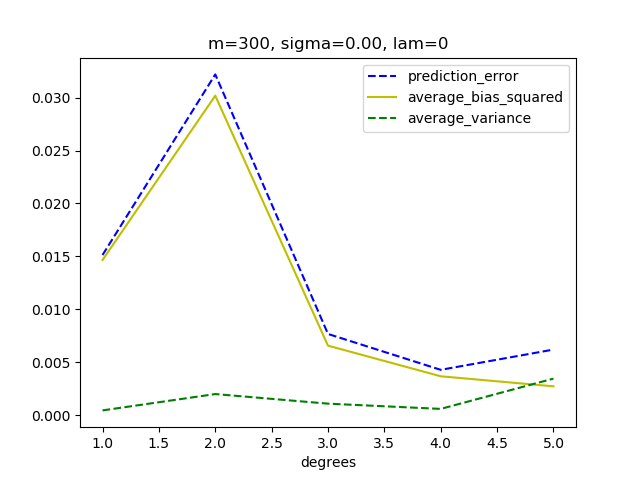
\includegraphics[width=1\textwidth]{plot_ols_without_r2/olsprediction_error_vs_degrees_m300_l300_s0.png}
	
	\caption{This shows the bias-variance tradeoff as function of the maximum polynomial degree used in the OLS method, with a sample size of 300.}
	\label{fig:1}
\end{figure}
\FloatBarrier

\medskip

\FloatBarrier
\begin{figure}[!ht]
	\centering
	\FloatBarrier
	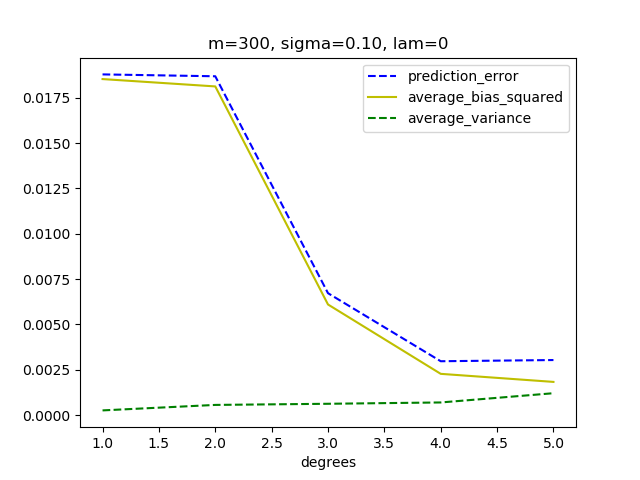
\includegraphics[width=1\textwidth]{plot_ols_without_r2/olsprediction_error_vs_degrees_m300_l300_s10.png}
	
	\caption{This shows the bias-variance tradeoff as function of the maximum polynomial degree used in the OLS method, with a sample size of 300 and a random gaussian noise with standard deviation of 0.1.}
	\label{fig:1}
\end{figure}
\FloatBarrier

\medskip

\FloatBarrier
\begin{figure}[!ht]
	\centering
	\FloatBarrier
	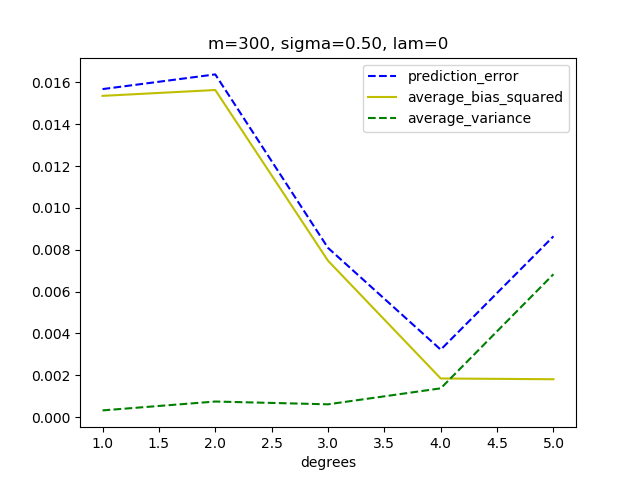
\includegraphics[width=1\textwidth]{plot_ols_without_r2/olsprediction_error_vs_degrees_m300_l300_s50.png}
	
	\caption{This shows the bias-variance tradeoff as function of the maximum polynomial degree used in the OLS method, with a sample size of 300 and a random gaussian noise with standard deviation of 0.5.}
	\label{fig:1}
\end{figure}
\FloatBarrier

\medskip

\subsubsection{Ridge}

Below are the figures for varying sample sizes, degree of polynomials and penalty with Ridge.

\FloatBarrier
\begin{figure}[!ht]
	\centering
	\FloatBarrier
	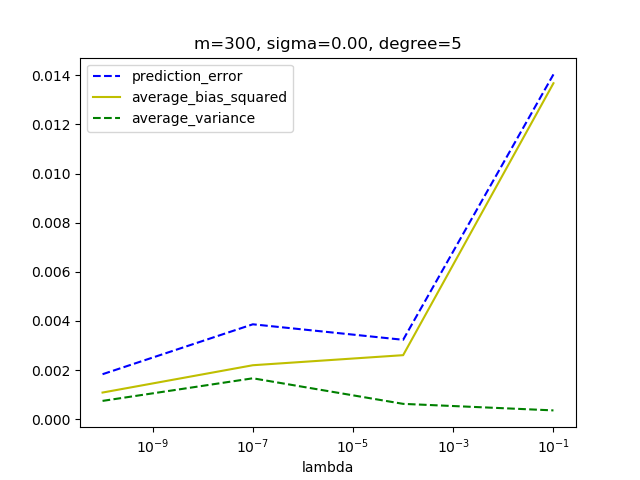
\includegraphics[width=1\textwidth]{plot_ridge_without_r2/ridgeprediction_error_m300_d5_s0.png}
	
	\caption{This shows the bias-variance tradeoff as function of the regularization parameter, lambda,for Ridge regression with a sample size of 300 and a polynomial degree of 5}
	\label{fig:2}
\end{figure}
\FloatBarrier

\medskip


\FloatBarrier
\begin{figure}[!ht]
	\centering
	\FloatBarrier
	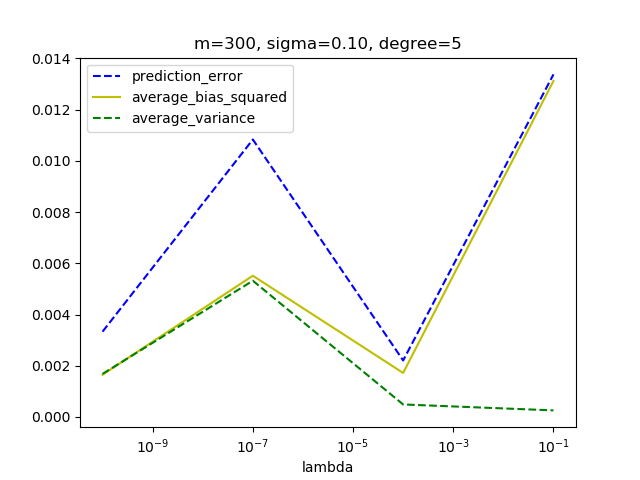
\includegraphics[width=1\textwidth]{plot_ridge_without_r2/ridgeprediction_error_m300_d5_s10.png}
	
	\caption{This shows the bias-variance tradeoff as function of the regularization parameter, lambda,for Ridge regression with a sample size of 300, polynomial degree of 5 and standard deviation of 0.1}
	\label{fig:2}
\end{figure}
\FloatBarrier

\medskip

\FloatBarrier
\begin{figure}[!ht]
	\centering
	\FloatBarrier
	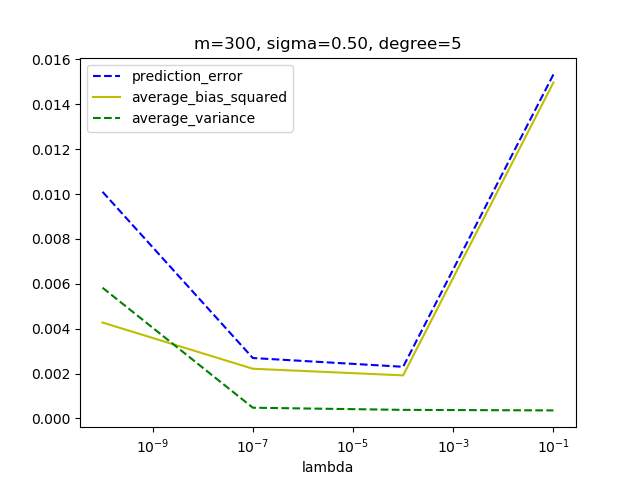
\includegraphics[width=1\textwidth]{plot_ridge_without_r2/ridgeprediction_error_m300_d5_s50.png}
	
	\caption{This shows the bias-variance tradeoff as function of the regularization parameter, lambda,for Ridge regression with a sample size of 300, polynomial degree of 5 and standard deviation of 0.5}
	\label{fig:2}
\end{figure}
\FloatBarrier

\medskip



\subsubsection{Lasso}
Below are the figures for varying sample sizes, polynomials and penalty with Lasso.
\FloatBarrier
\begin{figure}[!ht]
	\centering
	\FloatBarrier
	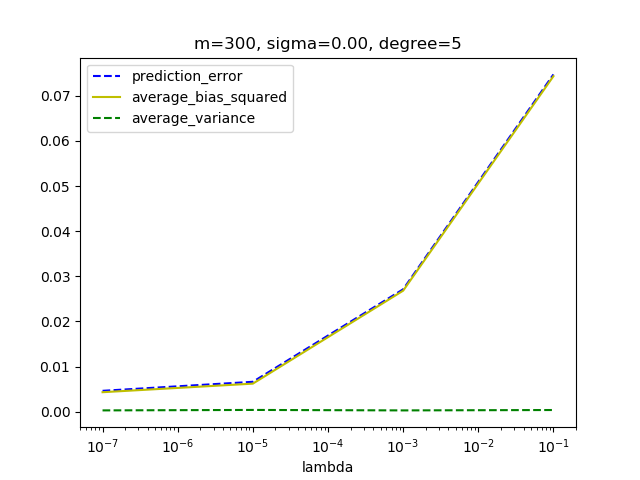
\includegraphics[width=1\textwidth]{lasso_prediction_vs_lambda/lassoprediction_error_m300_d5_s0.png}
	
	\caption{This shows the bias-variance tradeoff as function of the regularization parameter, lambda, for Lasso regression method with a sample size of 300 and a polynomial degree of 5}
	\label{fig:3}
\end{figure}
\FloatBarrier

\medskip

\FloatBarrier
\begin{figure}[!ht]
	\centering
	\FloatBarrier
	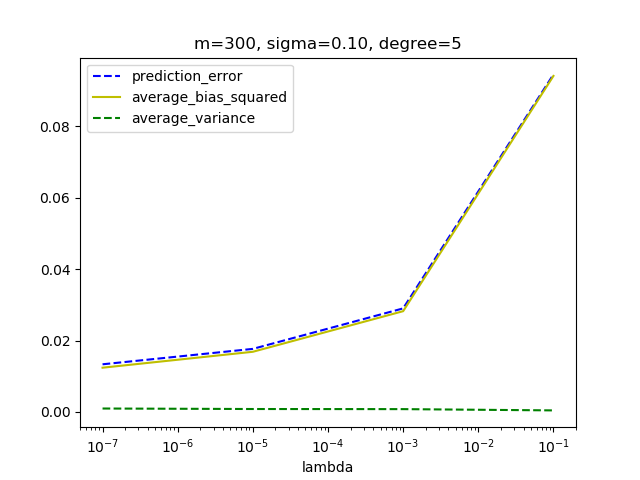
\includegraphics[width=1\textwidth]{lasso_prediction_vs_lambda/lassoprediction_error_m300_d5_s10.png}
	
	\caption{This shows the bias-variance tradeoff as function of the regularization parameter, lambda, for Lasso regression method with a sample size of 300, polynomial degree of 5 and standard deviation of 0.1.}
	\label{fig:3}
\end{figure}
\FloatBarrier

\medskip

\FloatBarrier
\begin{figure}[!ht]
	\centering
	\FloatBarrier
	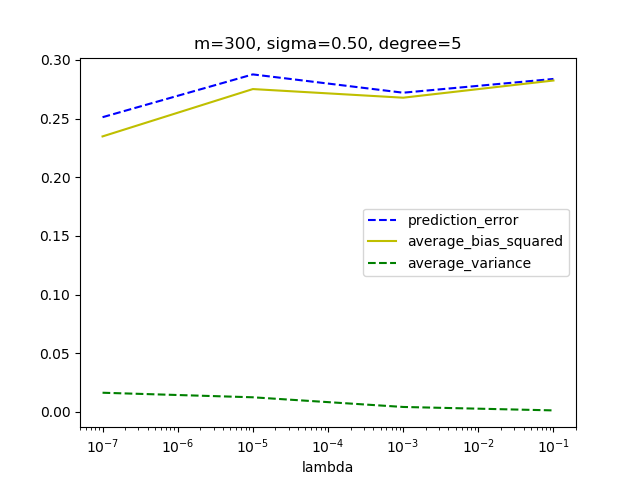
\includegraphics[width=1\textwidth]{lasso_prediction_vs_lambda/lassoprediction_error_m300_d5_s50.png}
	
	\caption{This shows the bias-variance tradeoff as function of the regularization parameter, lambda, for Lasso regression method with a sample size of 300, a polynomial degree of 5 and standard deviation of 0.5}
	\label{fig:3}
\end{figure}
\FloatBarrier

\medskip

\subsection{Discussion}
From all the figures I will now consider prediction error, bias and variance for the various methods.

\subsubsection{OLS}
For the OLS I can see that the minimum prediction error is for a polynomial of degree 4 for all standard deviations 0, 0.1 and 0.5. IN all cases the value of the prediction error is about 0.004. The bias is smallest at 5 degrees in all cases. The variance is smallest for a degree 4 polynomial for standard deviations of 0 and 0.1. For standard deviation of 0.5 the smallest variance is at 3. For a degree 1 polynomial, we do have a low variance, but the bias is really high.
\medskip

Table \ref{Table:1} shows that there were only 5 significant coefficients, the other ones could possibly have been set to 0, but that was not implemented. In principle I could have found a best subset model here.

\subsubsection{Ridge}
For the ridge regression I can see a low prediction error for lambda being $10^{-4}$ and $10^{-10}$ for the 0 and 0.1 standard deviation cases, with a value of the prediction error of about 0.0035 and 0.002. The lowest value being for 0.1 standard deviation and lambda $10^{-4}$. For the 0.5 standard deviation case, the prediction error is the smallest at about 0.25 for lambda $10^{-4}$.

\subsubsection{Lasso}
For the lasso regression at standard deviation of 0 I can see a minimum prediction error of about 0.005 for lambda $10^{-7}$. For standard deviation 0.1 the prediction error is up to 0.015 and for standard deviation 0.5 it is all the way up to 0.25. This tells me that something might have gone wrong with the implementation of lasso. 

\section{Conclusion}

The results show that the Ridge regression gives a better prediction error than the other two methods. That does not agree with the expected, since the Lasso method should have been better. I tried to figure out the reason why that happened, and I came up with the following explanation:

The formulation of Lasso is the same as for Ridge, but for the extra $\beta$ term in Ridge. It seems clear from the results that the Ridge method was to be preferred, but on further inspection, it seemed that the Lasso method may have been worse because the standardization method was not done correctly for Lasso. I suspect this was the reason for Lasso being worse than the Ridge regression.

I then implemented this standardization, and still found that the Lasso regression was inferior to the ridge regression, which I can not fully explain.


\section*{Improvements}
I would have liked to complete the data analysis, and also figured out why Ridge regression showed superior results compared to the Lasso Regression. For the OLS method I could have found a best subset model after having found the significant coefficients.


\section{Bibliography}
\begin{thebibliography}{99}
	\bibitem{projecttext}$\href{https://github.com/CompPhysics/MachineLearning/blob/master/doc/Projects/2018/Project1/pdf/Project1.pdf}{https://github.com/CompPhysics/MachineLearning/blob/master/doc/Projects/2018/Project1/pdf/Project1.pdf}$
	
	\bibitem{elementsstat}$\href{https://github.com/CompPhysics/MachineLearning/blob/master/doc/Textbooks/elementsstat.pdf}{https://github.com/CompPhysics/MachineLearning/blob/master/doc/Textbooks/elementsstat.pdf}$
	
	\bibitem{ridge}$\href{https://arxiv.org/pdf/1509.09169.pdf}{https://arxiv.org/pdf/1509.09169.pdf}$
	
	\bibitem{franke}$\href{http://www.dtic.mil/dtic/tr/fulltext/u2/a081688.pdf}{http://www.dtic.mil/dtic/tr/fulltext/u2/a081688.pdf}$
	
	
\end{thebibliography}
